\section{Product architecture}
Our product consists of a plug-in developed for the Grafana platform and a Training Tool external to this platform. Therefore the analysis of the architecture is divided into these two components.

\subsection{Training tool}
The Training tool deals with training an SVM or LR algorithm using a dataset inserted by the user, to then generate a JSON file containing the necessary information to perform the prediction. This module has been developed following the \textit{MVVM} behavioral design pattern.

\subsubsection{Architectural design}
We decided to implement this pattern because React\glo was used to build the component and we believed that this pattern coupled well with the structure of the latter. Moreover, it allows to divide the \textit{Presentation Logic}\glo and the \textit{Business Logic}\glo and it allows to reuse some components in other contexts, without having to change them.

As can be seen in the following figure, we have the View that exchanges information on user interactions with the ViewModel, which in turn transforms them into actions on the data performed by the Model.
The data transition from the View to the Model occurs through the modification of a \texttt{props} data field entered by the ViewModel. Through these props, the ViewModel calls the correct functions when the user interacts with the View. The division between Business Logic and Presentation Logic is reinforced by this use of props. The Model provides functionality for the management of the algorithms through the \texttt{SVMtrain} and \texttt{RLtrain} classes that will be used by the ViewModel. 
Finally there is a communication between Model and View for the constant updating of the latter, thanks to a functionality provided by the Grafana platform.

\begin{figure}[H]
\centering
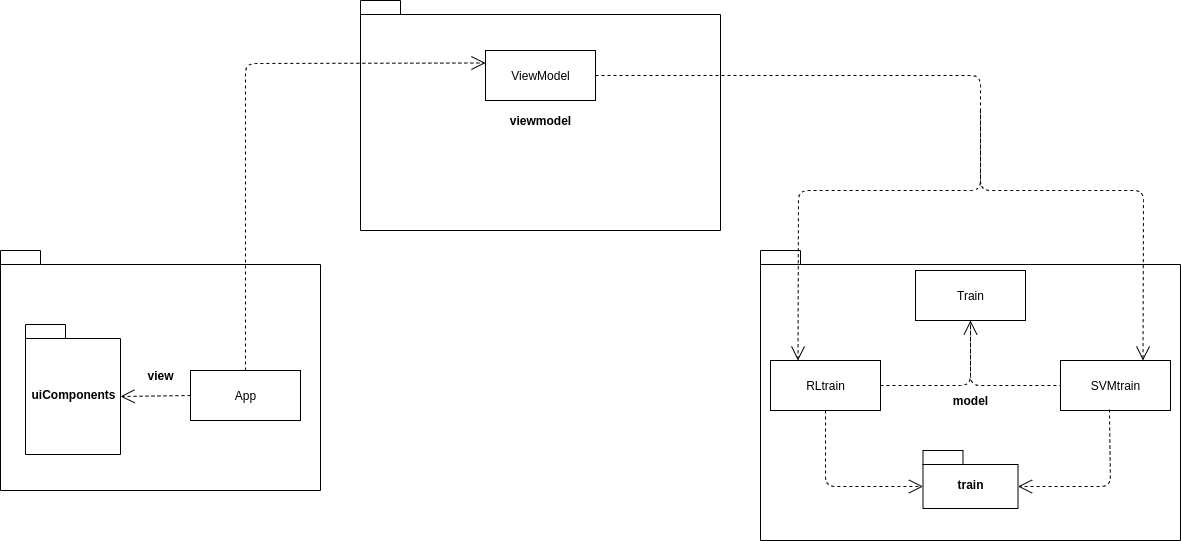
\includegraphics[scale=0.4]{../../../Diagrams/Package_diagrams/tool_design_patern.png}
\caption{Training tool package diagram}
\end{figure}

Analyzing the specific components, our architecture is structured as follows:
\begin{itemize}
\item \textbf{Model}: it manages the \textit{business logic}. It contains
the data prediction algorithms that have been presently implemented and writing the result of the predictions to an Influx database;
\item \textbf{View}: it manages the \textit{presentation logic}. It allows the creation of a customized graphic panel within a Grafana dashboard. With this panel the user can select prediction algorithm settings, incoming data streams and the minimum and maximum thresholds;
\item \textbf{ViewModel}: it manages the \textit{application logic}\glo. The ViewModel is an abstraction of the view exposing public properties and commands. MVVM has a binder, which automates communication between the View and its bound properties in the ViewModel.
\end{itemize}

\paragraph{Grafana's role}\mbox{} \\ \mbox{} \\
Grafana plays a fundamental role in the architecture as it allows continuous updating of the View to change the data in the Model. In particular, whenever there are updates on the data in the Model, Grafana makes them available to View through specific methods, together with the configuration of the queries with which this data was obtained. Moreover, through React, it manages the two-way data binding between HTML View and Javascript code, in addition to offering most of the necessary graphic components for the realization of the plug-in View.

\subsubsection{Detail design}

\paragraph{Model}\mbox{} \\ \mbox{} \\
The main component of the Model is the abstract class of the prediction algorithms called Train. Starting with this, we have implemented
two algorithms: Support Vector Machine and Linear Regression.
They are represented respectively by the concrete classes \texttt{SupportSVM}
and \texttt{SupportRL}. We have found that, for families algorithms such as Support Vector Machine and Linear Regression algorithms, it is possible to trace them to a single abstract class as we have provided. 

\paragraph*{Train}\mbox{} \\ \mbox{} \\
The abstract class of the prediction algorithms is called \texttt{Train} and it
represents the contract that all concrete classes must abide to be able to characterize a prediction algorithm. It contains only one parameter: \texttt{algorithm}. The \texttt{train()} method allows you to perform the prediction on a specific dataset. The \texttt{getJSON()} method writes the configuration parameters into the JSON file.

\paragraph*{SupportSVM}\mbox{} \\ \mbox{} \\
To implement the Support Vector Machine algorithm we developed the concrete class \texttt{SupportSVM}. This class performs the prediction on the dataset. 
It also makes use of components specific to the SVM class imported from the SVM library to perform the real prediction. SupportSVM also contains two fields data: \begin{itemize}
\item dataSVM: reference to the dataset;
\item weights: the weights are the SVM coefficients that will be used to make the prediction.
\end{itemize}
Finally, there is the constructor that allows you to run the method binding to the class.

\paragraph*{SupportRL}\mbox{} \\ \mbox{} \\
To implement the Linear Regression algorithm we developed the concrete class \texttt{SupportRL}. This class performs the prediction on the dataset. It also makes use of components specific to the RL class imported from the RL library to perform the real prediction. SupportRL also contains two fields data: \begin{itemize}
\item dataRL: reference to the dataset;
\item numOfX: the numbers of X founded on the CSV file;
\item coefficients: the coefficients needed to make the prediction.
\end{itemize}
Finally, there is the constructor that allows you to run the method binding to the class.

\begin{figure}[H]
\centering
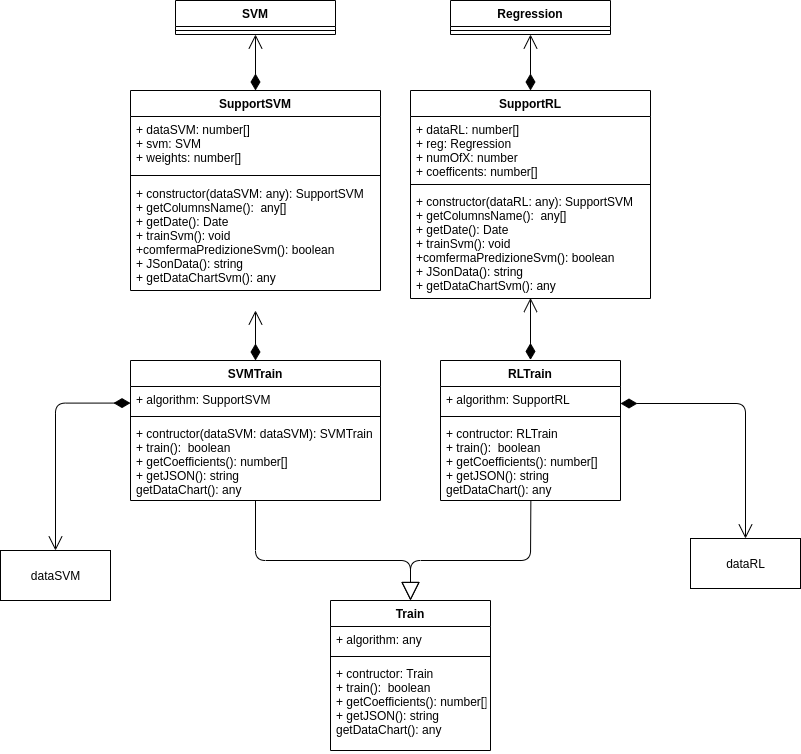
\includegraphics[scale=0.5]{../../../Diagrams/Classes_diagrams/tool_model.png}
\caption{Training tool Model class diagram}
\end{figure}

\paragraph{View}\mbox{} \\ \mbox{} \\
Inside the View there are all the view components.
The \texttt{App} class is the main component and it represents the tool's entry point. Each part of the View has been divided into components and rendered by the App. The communication between these components and the App takes place through the \texttt{props} (conceptually, the components are like JavaScript functions): it accepts arbitrary data (under the name of "props") and returns React elements that describe what should appear on the screen.
Inside there is an instance of the ViewModel for data-binding.

\subparagraph*{App}\mbox{} \\ \mbox{} \\
The \texttt{App} class is the main component and it represents the tool's entry point. Each part of the View has been divided into components and rendered by the App. This class has just one parameter: \texttt{viewModel} in an instance of the ViewModel. The constructor contains the properties in common with the ViewModel. Moreover, it has the following methods:
\begin{itemize}
\item \texttt{changeAlgorithm(event)}: it manages the algorithm user's choice, setting the \texttt{algorithm} state value after the event was made;
\item \texttt{resetAlgorithm(algorithm)}: it sets the \texttt{algorithm} state parameter to the default value;
\item \texttt{setDataFromFile(data, fileInfo)}: it sets the \texttt{data} state parameter and the \texttt{fileName} state parameter with the inserted file's name;
\item \texttt{handleTraining()}: it sends the data to the ViewModel and if the \texttt{performTraining()} method success, it calls the function to write the information into the JSON file, otherwise it resets the algorithm and sets the \texttt{jsonData} to null;
\item \texttt{downloadJsonData()}: it creates the DownloadJson component;
\item \texttt{render()}: it creates the InsertCsvButton, ComboBoxAlgorithm, TrainButton and Chart components and it calls the \texttt{downloadJsonData()} function.
\end{itemize}	

\subparagraph*{combo\_box\_algorithm}\mbox{} \\ \mbox{} \\
It renders the combo box for the algorithm's choice.\\
The \texttt{render()} method renders the JSX\glo element wanted.

\subparagraph*{download\_json}\mbox{} \\ \mbox{} \\
It manages and render the "Download" button.\\
The \texttt{downloadJsonFile()} method allow to download the file, making the connection between the browser and the local pc.
The \texttt{render()} method renders the "Download" button.

\subparagraph*{chart}\mbox{} \\ \mbox{} \\
It renders the chart.
This component contains the following parameters: 
\begin{itemize}
\item data: contains the data that must be shown;
\item options: contains the various option that can be apply to the graph, such as colors, axes and the regression line.
\end{itemize}
It also implements the following methods: 
\begin{itemize}
\item \texttt{RLChart{}}: it contains the methods to print the graphic of a rl-trained file on the screen; 
\item \texttt{SVMChart()}: it contains the methods to print the graphic of a svm-trained file on the screen;
\item \texttt{formatData()}: it associates and manages the data to the graph;
\item \texttt{render()}: it renders the chart graph.

\end{itemize}

\subparagraph*{insert\_csv\_button}\mbox{} \\ \mbox{} \\
It renders the insert button for the CSV file.\\
The \texttt{render()} method renders the "Inserisci file" button.

\subparagraph*{header}\mbox{} \\ \mbox{} \\
It renders the header.\\
The \texttt{render()} method renders the site's header.

\subparagraph*{train\_button}\mbox{} \\ \mbox{} \\
It renders the train button, that will start the training.\\
The \texttt{render()} method renders the "Conferma" button.

\begin{figure}[H]
\centering
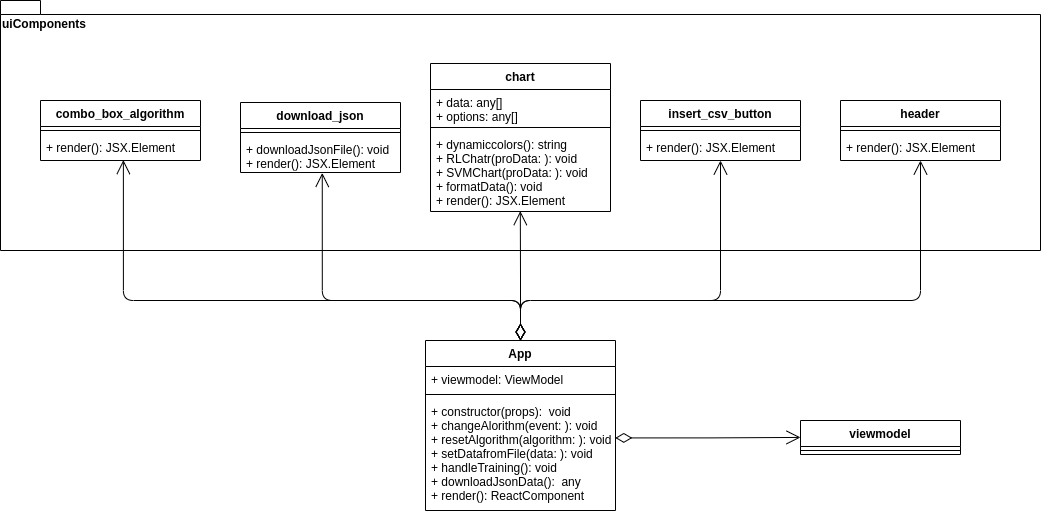
\includegraphics[scale=0.45]{../../../Diagrams/Classes_diagrams/tool_view.png}
\caption{Training tool Model class diagram}
\end{figure}



